%%%%%%%%%%%%%%%%%%%%%%%%%%%%%%%%%%%%%%%%%%%%%%%%%%%%%%%%%%%%%%%%%%%%%%%%%%%%%%%
%%%%%%%%%%%%%%%%%%%%%%%%%%%%%%%%%%%%%%%%%%%%%%%%%%%%%%%%%%%%%%%%%%%%%%%%%%%%%%%
\section{Methods for Analyzing Spatial Proximity Networks}
%%%%%%%%%%%%%%%%%%%%%%%%%%%%%%%%%%%%%%%%%%%%%%%%%%%%%%%%%%%%%%%%%%%%%%%%%%%%%%%
%%%%%%%%%%%%%%%%%%%%%%%%%%%%%%%%%%%%%%%%%%%%%%%%%%%%%%%%%%%%%%%%%%%%%%%%%%%%%%%
This section outlines the methods I used to investigate the networks on a global, intermediate and local level.
It explains the choice of network measures used for the global analysis.
Also, I report the decision for a community detection algorithm and illustrate the methods to examine the segregation of communities concerning age and spatial distribution.
Furthermore, I explain what approach I used to study the development of communities.

%%%%%%%%%%%%%%%%%%%%%%%%%%%%%%%%%%%%%%%%%%%%%%%%%%%%%%%%%%%%%%%%%%%%%%%%%%%%%%%
\subsection{Investigating the Topology and Network Characteristics}
\label{subsec:APmeasures}
%%%%%%%%%%%%%%%%%%%%%%%%%%%%%%%%%%%%%%%%%%%%%%%%%%%%%%%%%%%%%%%%%%%%%%%%%%%%%%%
I summarized the network analysis methods of the reviewed studies (chapter~\ref{ch:relatedwork}) to gain an overview of established procedures in the field of social insect networks. I grouped the methods by global measures, node level measures and other network analysis methods.
Table~\ref{tab:study-measures} summarizes the used network analysis methods of the reviewed studies.
The network measures I chose for the global and node level analysis are listed in table~\ref{tab:netprop} and were defined in chapter~\ref{sec:definitions}.

Each link in the network is attributed with the frequency of interactions and total duration of interactions between the two individuals.
Figure~\ref{fig:fVSd} shows a strong positive correlation between those two values. For further analysis I decided to use the frequency of interactions as the weight for links, analogously to \cite{mersch2013tracking,baracchi2014socio}.


\begin{figure}[htb]
	\centering
	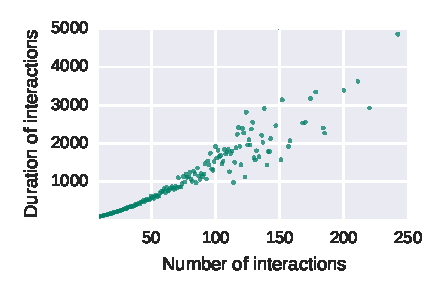
\includegraphics[width=1.0\textwidth]{Figures/n3-freqVSduration}
	\caption[Frequency and total duration of interaction]{\textbf{Frequency and total duration of interaction} The two link weight values show a strong positive correlation. The data of the three snapshots is aggregated.}
	\label{fig:fVSd}
\end{figure}

The degree of a bee represents the number of other bees this focal animal interacts.
Bees with a high number of interaction partners, have a high degree.
This measure was chosen because it reveals a lot about the general topology of a network.
The strength of a bee is the sum of its link weights. A high strength refers either to a large number of interaction partners with a low link weight or a low number of interaction partners with high link weights. Especially for aggregated networks this measure accumulates valuable information regarding the interaction activity of bees.
The local clustering coefficient (lcc) of a bee indicates how close its interaction partners are to being a clique\footnote{A clique is a complete subgraph.}. A large lcc shows that most of its interaction partners interact with each other. A low lcc indicates the absence of those interactions.
It is a good indicator for the embeddedness of single bees.

The betweenness of a bee measures, how many shortest paths go through that bee. A bee with a high betweenness would be central or important for the network in the sense of information flow. Removing this bee from the hive would lead to the breakdown of information or food flow and would negatively affect the robustness of the network.
The closeness of a bee measures how fast this bee can reach all others in the network. A high closeness would indicate a very short path to every other bee. Regarding information flow, a bee with high closeness can spread e.g. information to all other bees very fast.
I selected these centrality measures exemplarily.

I examined all node level metrics concerning the age of bees and their detection frequency. The global network properties are compared to an Erd\H{o}s-R\'{e}niy  random network, by averaging over 100 runs.

\begin{table}
\small
\centering
\caption[Measures used for analysis]{\textbf{Measures used for analysis} Each measure is explained in chapter~\ref{sec:definitions}}
\vspace*{5mm}
\begin{tabularx}{\textwidth}{p{0.5\linewidth}p{0.5\linewidth}}
\toprule
Global level measures & Node level measures\\
\midrule
Number of nodes $N$ and edges $E$ & Degree $k$ \\
Average degree $\langle k \rangle$ &  Strength $s$\\
Average strength $\langle s \rangle$ &   Local clustering coefficient $c$\\
Density $D$ & Closeness Centrality $C_C$ \\
Diameter $d_{max}$ & Betweenness Centrality $C_B$\\
Number of components & \\
Global clustering coefficient $C_{\Delta}$ &  \\
Average path length $\langle d \rangle$ & \\
Edge weights & \\

\bottomrule
\end{tabularx}
\label{tab:netprop}
\end{table}


%%%%%%%%%%%%%%%%%%%%%%%%%%%%%%%%%%%%%%%%%%%%%%%%%%%%%%%%%%%%%%%%%%%%%%%%%%%%%%%
\subsection{Detecting Communities}
\label{subsec:APcommunityDet}
%%%%%%%%%%%%%%%%%%%%%%%%%%%%%%%%%%%%%%%%%%%%%%%%%%%%%%%%%%%%%%%%%%%%%%%%%%%%%%%
For finding an appropriate community detection algorithms, I checked the reviewed studies for applicable methods and scanned papers, which compare various community detection algorithms. Finally, I checked a subset of algorithms, which I identified as suitable in this context.

The reviewed studies only include two examples of community respectively cluster analysis. \textcite{mersch2013tracking} used the infomap~\cite{rosvall2009map,rosvall2007information} algorithm. According to the authors, this algorithm only works with sparse networks and is therefore not applicable in my case of densely connected spatial proximity networks. \textcite{baracchi2014socio} use a hierarchical clustering to infer groups of bees within the network that are similar regarding the measures strength, eigenvector, and betweenness centrality. In contrast to the resulting groups of community detection, groups identified by hierarchical clustering do not automatically refer to dense subgraphs of the network.

Much literature on the comparative analysis of community detection algorithms exist, e.g.~\cite{yang2016comparative, harenberg2014community}. Some studies seem to be promising, but assume either a power law degree distribution or
evaluate networks with a low density, which is not applicable here.
Thererfore, I tested community detection algorithms implemented in python, to find an algorithm, which works well for my case of animal social networks. The three most common python libraries for network analysis were reviewed: NetworkX\footnote{\url{https://networkx.github.io/}; Last accessed: 16.03.2016, 6:36~p.m.}, igraph\footnote{\url{http://igraph.org/python/}; Last accessed: 16.03.2016, 6:38~p.m.}, and graph-tool\footnote{\url{https://graph-tool.skewed.de/}; Last accessed: 16:03.2016, 6:39~p.m.})
The algorithm needs to fulfill the following criterias:

\begin{itemize}
\item Support for large and very dense networks ($N=1000$, $D>50\%$)
\item Support for weighted link
\item Fast runtime
\end{itemize}

Table~\ref{tab:algos} gives an overview about the algorithms reviewed. Five algorithms did not terminate after 15~minutes and were therefore excluded from further investigations. Infomap and label propagation tend to partition all nodes into a single community, this is known especially in dense graphs~\cite{yang2016comparative, fortunato2010community}.
The Louvain algorithm~\footnote{Implemented in python for networkX: \url{http://perso.crans.org/aynaud/communities/api.html}} (networkX) is the same as multilevel (iGraph), but takes longer producing almost the same communities and therefore was also excluded. Walktrap was tested for different step size parameters, as suggested in~\cite{pons2005computing}, the communities remained almost the same, only a few nodes switched communities.

I examined the number and size of detected communities for the algorithms fastgreedy, leading eigenvector, multilevel, and walktrap for all three snapshots. Table~\ref{tab:algos4} gives an overview about the results.
All algorithms found at least two communities.
Except for leading eigenvector, most tend to find three communities.

I decided to use two algorithms for community detection: leading eigenvector and walktrap. \textcite{farine2015constructing} explains that leading eigenvector is often used with animal social networks and works well. Walktrap is chosen for also examining the third community.

\begin{table}[htbp]
\small
\caption[Compairing community detection algorithms]{\textbf{Comparing community detection algorithms} Comparison of algorithms implemented in python. Criterias are the support of weighted edges, runtime and number of communities. A runtime indicated by $-$ mean no termination after 15~minutes.\\
}
\label{tab:algos}

\begin{tabularx}{\textwidth}{lcccccccccccc}
\toprule
	 {} &
	 \rotatebox{90}{\textbf{fastgreedy$^1$}} &
	 \rotatebox{90}{\textbf{leading eigenvector$^1$}} &
	 \rotatebox{90}{louvain$^2$} &
	 \rotatebox{90}{\textbf{multilevel$^1$}} &
	 \rotatebox{90}{\textbf{walktrap$^1$}} &
	 
	 \rotatebox{90}{infomap$^1$} &
	 \rotatebox{90}{label propagation$^1$} &
	 
	 \rotatebox{90}{edge betweenness$^1$} &
	 \rotatebox{90}{k-clique communities$^2$\thinspace} &
	 \rotatebox{90}{optimal modularity$^1$} &
	 \rotatebox{90}{spinglass$^1$} &
	 \rotatebox{90}{statistical inference$^3$} \\ \midrule
	 
	 
	 
	 Edge weights & $\times$ & $\times$ & $\times$ & $\times$ & $\times$ & $\times$ & $\times$ & & $\times$ & $\times$ & $\times$ \\ \midrule
	 Runtime in sec & ~$3.6$ & ~$6.3$ & $11.7$ & ~$0.7$ & $19.4$ & $13.2$ & ~$0.2$ & $-$ & $-$ & $-$ & $-$ & $-$ \\ \midrule
	 Communities & $3$ & $2$ & $2$ & $3$ & $2$ & $1$ & $1$ & $-$ & $-$ & $-$ & $-$ & $-$ \\ \midrule
	  & 473 & 488 & 469 & 462 & 490 & 922 &  922 &  &  &  &  &  \\
	  & 434 & 434 & 453 & 427 & 431 &  &  &  &  &  &  &  \\
	  & 15 &  &  & 33 & (1) &  &  &  &  &  &  &  \\
	 \bottomrule
	 
\end{tabularx}
\begin{flushright}
\footnotesize{
$^1$ igraph, $^2$ NetworkX, $^3$ graph-tool\\
}
\end{flushright}

\end{table}

% \hdashline
% \midrule
% \bottomrule
\begin{table}[htbp]
\centering
\caption[X]{\textbf{X} X\\
}
\label{tab:algos4}

\begin{tabular}{lcccc}
\toprule
	 {} &
	 fastgreedy &
	 leading eigenvector &
	 multilevel &
	 walktrap \\ \midrule
	 
	  Network 1
	  & 473 & 488 & 462 & 490 \\
	  & 434 & 434 & 427 & 431 \\
	  & 15 &   & 33 & (1) \\ \midrule
	  Network 2
	  & 504 & 503 & 481 & 372 \\
	  & 467 & 475 & 439 & 311 \\
	  & 7 &   &  58 & 294 \\
	  & & & & (1) \\ \midrule
	  Network 3
	  & 534 & 537 & 505 & 310 \\
	  & 388 & 385 & 415 & 390 \\
	  &  &   &  (2) & 231 \\
	 \bottomrule
	 
\end{tabular}

\end{table}

% \hdashline
% \midrule
% \bottomrule

\subsubsection{Age and Spatial Distribution of Communities}
To answer the question whether communities reflect different age groups, I studied the average age and the general age distribution of communities. I also investigated whether the age division persists in each snapshot. A two-sample Kolmogorov-Smirnov test was used to determine the statistical difference of the age distribution between communities.

To investigate whether communities reflect groups of bees working in different areas of the comb, I used heat maps to determine the core regions per group and snapshot visually.
I stored the positions of all bees present within the ten hour time windows in an SQLite database to faster access the data and to eliminate the time-consuming parsing.

%%%%%%%%%%%%%%%%%%%%%%%%%%%%%%%%%%%%%%%%%%%%%%%%%%%%%%%%%%%%%%%%%%%%%%%%%%%%%%%
\subsection{Development of Community Members}
\label{sec:bg:tracking}
%%%%%%%%%%%%%%%%%%%%%%%%%%%%%%%%%%%%%%%%%%%%%%%%%%%%%%%%%%%%%%%%%%%%%%%%%%%%%%%
According to \textcite{aynaud2013communities} and  \textcite{brodka2014community} there are three main approaches for community detection in temporal networks (sometimes referred to as community tracking): (1) using a static community detection algorithm on several snapshots and then solving a matching problem, (2) using algorithms that are directly suited for temporal networks and (3) using incremental or online algorithms when processing data streams. For each of the three approaches, several methods already exist.
As community tracking is not the main focus of this work, I chose to apply the most natural method out of approach (1): detecting static communities for each snapshot and then matching those communities using set theory.

Two communities at successive time steps are matched if they share enough nodes.
The \emph{match value} between two communities $C$ and $D$ according to \textcite{hopcroft2004tracking} is defined as:

\begin{equation}
\label{eq:match}
\texttt{match}(C,D) = \texttt{min}\left( \frac{\textbar C\cap D \textbar}{\textbar C\textbar }, \frac{\textbar C\cap D \textbar}{\textbar D \textbar }\right)
\end{equation}

This value is between 0 and 1. A high match value occurs when two communities share many nodes and are of a similar size. Communities with the highest value are matched, respectively represent the same community to different points in time. The author suggests applying a threshold to more precisely define what ``share enough nodes'' means. Otherwise, a matching could occur between communities with only 0.1\% of overlapping nodes.

To investigate the total number of bees, that remain in the network over the three snapshots, I inspected the match value of bees in consecutive snapshots. Also, I calculated all match values between communities in consecutive snapshots and additionally calculated the number of intersecting bees. I visualize the dynamic movement
of bees between groups of different snapshots with a flowchart diagram using the JavaScript library D3.js\footnote{\url{https://d3js.org/}}.